%---- using TikZ for drawing shapes
\documentclass{article}
\usepackage{tikz}

\title{Working with TikZ}
\author{Nima Poshtiban}
\date{\today}

\begin{document}
\maketitle

	
\begin{figure}[h] % using figure for more customizations
\centering
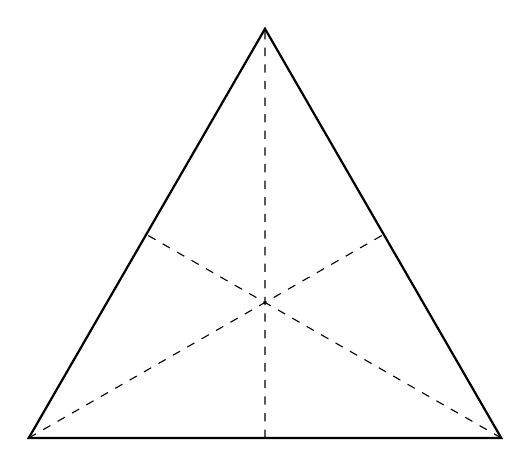
\begin{tikzpicture}[scale=3]
% "--" means to next coordinate
%---- (starting coordinates) -- (end coordinates) ;
%\draw (0,0) -- (2,0) ; % ---- the line must be end by ";"
\draw[thick] (0,0) -- (2,0) -- (1,{sqrt(3)}) -- cycle; %  "cycle"close the shape

% --- drawing multiple line using one draw command
\draw[dashed] (1,0) -- (1,{sqrt(3)}) (0,0) -- (1.5,0.86) (2,0) -- (0.5,0.86);

\end{tikzpicture}
\caption{A simple Triangle}
\end{figure}

\begin{figure}[h]
\centering
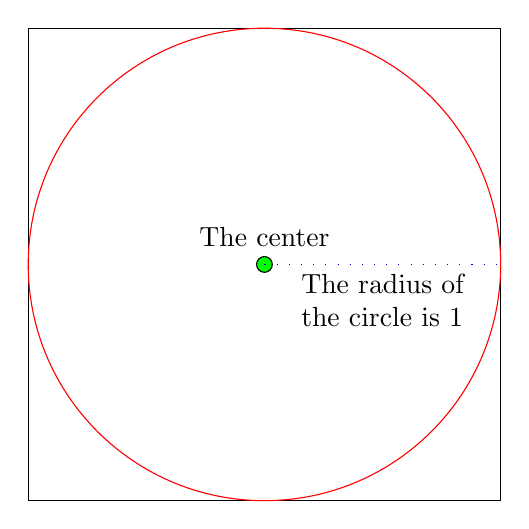
\begin{tikzpicture}
% --- making a rectangle
\draw (-3,-3) rectangle (3,3);
% ---- making a Circle
\draw[red] (0,0) circle [radius=3];

% ---- filled circle
\draw[fill=green] (0,0) circle [radius=0.1]; 
% ---- also you can use \fill instead

% --- a customized line 
\draw[blue,loosely dotted] (0,0) -- (3,0);

% ---- placing text in shape above the shape
\node[above] at (0,0.1){The center};

% ---- handling large text using alignment
\node[below,align=left] at (1.5,0) {
The radius of \\ the circle is 1};
\end{tikzpicture}
\caption{A Circle in a Rectangle}
\end{figure}

\begin{figure}
	% ------- making a plot
\centering
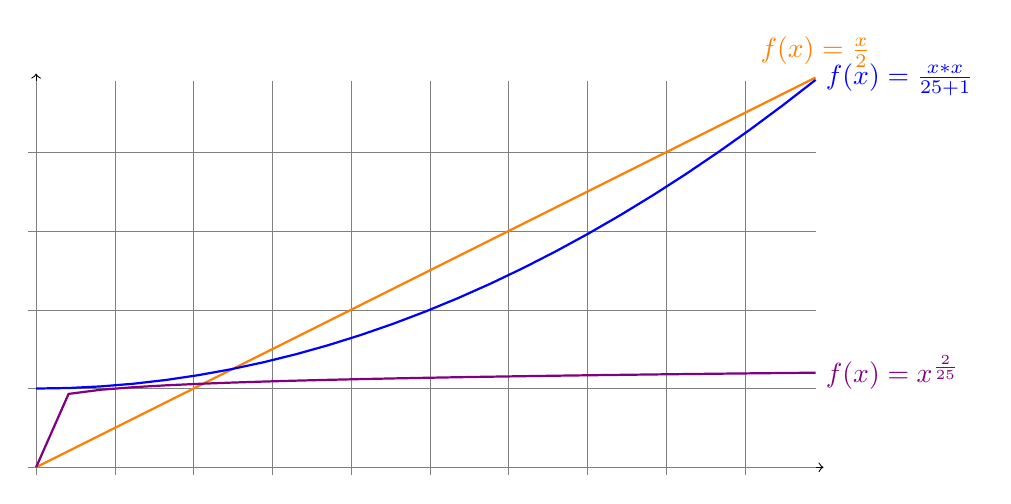
\begin{tikzpicture}[domain=0:9.9] 
\draw[->] (-0.1,0) -- (10,0); % --- x axis
\draw[->](0,-0.1) -- (0,5);  % y axix
\draw[gray,ultra thin] (-0.1,-0.1) grid (9.9,4.9); % drawing grid

\draw[orange,thick] plot (\x,\x/2) node[above,thick]{$f(x)=\frac{x}{2}$}; % --- plotting a function
% ----- node adds the text to function
\draw[blue,thick] plot (\x, \x * \x /25+1) node[right,thick]{$f(x)=\frac{x*x}{25+1}$}; % ---- another function

\draw[violet,thick] plot(\x, {pow(\x,2/25)}) node[right,thick]{$f(x)=x^{\frac{2}{25}}$}; % --- another function
\end{tikzpicture}
\caption{Plotting functions}
\end{figure}


\begin{figure}
\centering
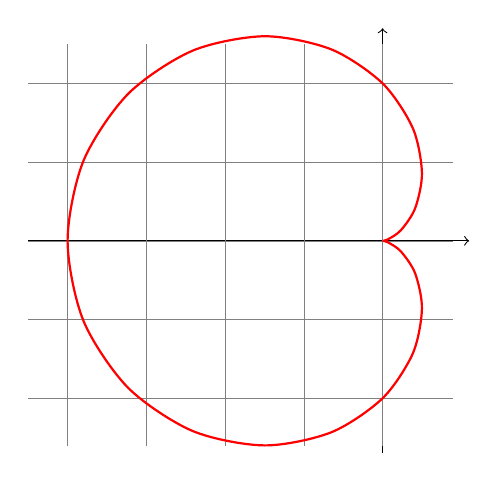
\begin{tikzpicture} %---- drawing curves
\draw[->] (0,-2.7) -- (0,2.7); % --- y axis
\draw[->] (-4.5,0) -- (1.1,0); % ---- x axis
\draw[gray,ultra thin] (-4.5,-2.6) grid (0.9,2.5) 
;
\draw[domain=0: 2*pi,smooth,red,thick] plot ({2*(1-cos(\x r) ) * cos(\x r)},{2*(1-cos(\x r))*sin(\x r)});
\end{tikzpicture}
\caption{Curves}
\end{figure}

\begin{figure}
\centering
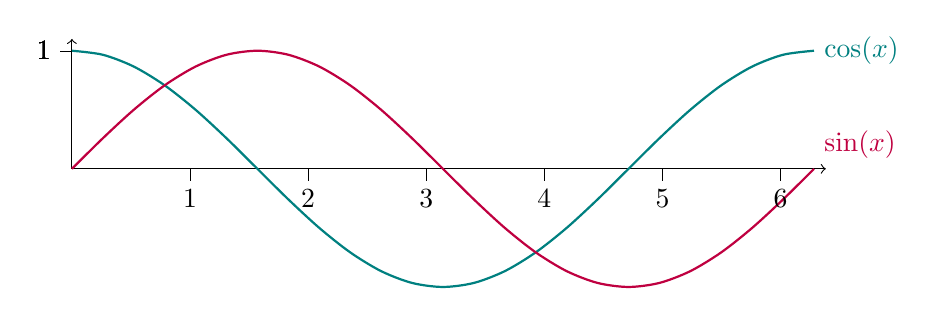
\begin{tikzpicture}[domain=0:2*pi,scale=1.5]
\draw[<->] (2*pi+0.1,0) -- (0,0) -- (0,1.1); % --- drawing x and y axis
\draw[smooth,teal,thick] plot (\x,{cos(\x r)}) node[right]{$\cos(x)$}; %---- f(x)=cos(x) 
\draw[smooth,purple,thick] plot (\x, {sin(
	\x r)}) node[above right]{$\sin(x)$}; % ----f(x)=sin(x)
%----- adding tick marks using for loop	
\foreach \x in {1,...,6}{
\draw[ultra thin] (\x,0) -- (\x,-0.1) node[below]{$\x$}; % x axis tick marks
\draw[ultra thin] (0,1) -- (-0.1,1) node[left]{$1$};
% y axis tick marks
}
\end{tikzpicture}
\end{figure}




\end{document}
